\begin{center}
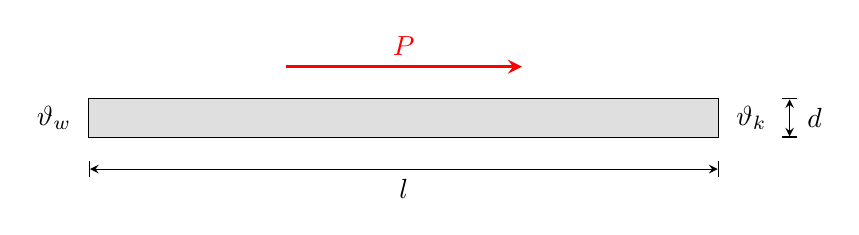
\begin{tikzpicture}[>=stealth]
 \draw[fill=gray!25] (0,0) rectangle (8,0.5);
 \node[anchor=east] at (-0.1,0.25) {$\vartheta_\text{w}$};
 \node[anchor=west] at (8.1,0.25) {$\vartheta_\text{k}$};
 \draw[->, very thick, red] (2.5,0.9) -- (5.5,0.9) node[midway, above] {$P$};
 \draw[|<->|] (0,-0.4) -- (8,-0.4) node[midway, below] {$l$};
 \draw[|<->|] (8.9,0) -- (8.9,0.5);
 \node[anchor=west] at (9.0,0.25) {$d$};
\end{tikzpicture}
\end{center}

Die Wärmeleitfähigkeit von Aluminium ist $\lambda = \lamO$ (FoTaBe S.~190). Der Temperaturunterschied zwischen den Enden ist $\Delta T = \dTF = \dT$. Nimmt man an, dass der Stab seitlich keine Wärme verliert, fliesst durch den Querschnitt $A = \pi d^2/4$ in der Zeit $t = \tsO$ die Wärme
\begin{align}
 Q &= \lambda\,A\,\frac{\Delta T}{l}\,t = \QsF \\
   &= \lam\cdot\frac{\pi\cdot\left(\dS\right)^2}{4}\cdot\frac{\dT}{\lS}\cdot\ts \\
   &= \Qs \approx \result{\QsP{0}{2}}
\end{align}
